\documentclass[11pt]{article}

\usepackage[margin=1in]{geometry}
\usepackage[T1]{fontenc}
\usepackage{lmodern}
\usepackage{microtype}
\usepackage{graphicx}
\usepackage{booktabs}
\usepackage{amsmath}
\usepackage[round]{natbib}
\usepackage[hidelinks]{hyperref}

\title{How Much History Does a Recommender Need?\\[0.3em]
\large Training-window length, quality and cost on the Netflix Prize ratings}
\author{Navya S G}
\date{November 2026}

\begin{document}
\maketitle

\begin{abstract}
Collaborative filtering models are usually trained on all the history a service has kept,
although tastes and catalogues change and training cost grows with every month retained. We ask
how much history three recommenders actually need. Popularity, Spark preference ALS and a
two-tower neural model are trained on windows of 1 to 24 months and on all history before three
monthly cutoffs in 2005, and are scored on the following month of the Netflix Prize ratings with
NDCG@10 against the full catalogue. Every plan was registered before it ran. Popularity and ALS
do best on the most recent month: ALS on 1 month scores 1.68 times its all-history score and
trains in about an eighth of the time. The two-tower model needs about 6 months, which reach
98.0\% of its 12-month score, and no model gains from history beyond 12 months. The two-tower
model scores above both baselines at every window and test month. Two supporting studies measure
the systems around the models: Spark needed every thread of a 4-thread machine to beat a
single-threaded program, and the served model met a 100\,ms latency target up to 400 simultaneous
users on one laptop.
\end{abstract}

\section{Introduction}

A recommender that keeps every rating ever made pays for it twice. Training time grows with the
number of rows, and old ratings may describe tastes that users no longer hold or films that are
no longer watched \citep{koren2009temporal}. Yet the length of the training history is rarely
treated as a variable: models are trained on what is available, and evaluated on a random sample
of the same period.

This report treats history length as the variable under study. It asks how much interaction
history a collaborative filtering model needs, what each additional month costs in compute, and
whether a neural model needs more or less history than matrix factorisation. The setting is the
Netflix Prize data \citep{bennett2007netflix}, which has about 100 million dated ratings, so a
window can be cut at any month and its cost measured.

The contributions are:
\begin{itemize}
  \item a temporal comparison of three models over six training windows and three test months,
    with every window scored on the same users and the same removed films;
  \item a registered decision rule for ``history needed'' and its answer for each model;
  \item the cost of each window, and a check of whether storing data by month makes short
    windows cheaper to train;
  \item two supporting measurements, of Spark's scaling against a single-threaded baseline and
    of the served model under load, each with its hardware named.
\end{itemize}

\section{Related work}

\paragraph{Time in collaborative filtering.} \citet{koren2009temporal} showed on this dataset
that user and item biases drift, and modelled the drift explicitly. This work asks a simpler
question that such models leave open: if a model is not told about time, how much history should
it be given?

\paragraph{Evaluation.} \citet{ji2023leakage} show that random and leave-one-out splits let models
train on interactions from after the test point, and that model rankings change with the amount
leaked. \citet{krichene2020sampled} show that metrics computed against a sample of negative items
can reverse model orderings, so this work ranks the full catalogue. \citet{dacrema2019progress}
found that many neural recommenders did not beat well-tuned simple baselines, and
\citet{rendle2020ncf} that a dot product is hard to beat. Both motivate the strong baselines
here, including popularity over the most recent month.

\paragraph{Models.} ALS for explicit ratings \citep{zhou2008als} and for implicit preference
\citep{hu2008implicit} are standard matrix factorisation baselines. Two-tower models encode users
and items separately and score them with a dot product \citep{covington2016youtube}; the one here
is trained with an in-batch softmax and the popularity correction of \citet{yi2019sampling}.

\paragraph{Systems cost.} \citet{mcsherry2015cost} define COST, the configuration that
outperforms a single thread, and found that many distributed systems need many cores to beat one
competent thread. We measure Spark's COST for this ALS job.

\paragraph{Privacy.} \citet{narayanan2008deanon} re-identified subscribers in this dataset from a
few known ratings, which shapes how the data is handled here (Section~\ref{sec:ethics}).

\section{Data and method}

\paragraph{Data.} The four training files hold 100,480,507 ratings by 480,189 users of 17,770
films, dated from 1999-11-11 to 2005-12-31, with no duplicate user and film pairs. They are stored
as Parquet in one folder per rating month. Ratings are skewed towards the end: 53.0\% are from
2005, so a window's length says little about its size, and every result reports rows as well as
months. November and December 2005 are excluded from testing, because ratings held back for the
competition and an 88.6\% fall in new users between October and December distort them.

\paragraph{Split.} The test months are August, September and October 2005. For a test month
starting at cutoff $c$, a window of $m$ months trains on ratings from $c$ minus $m$ months up to
$c$, and the model is scored on ratings in the month after $c$. Windows are 1, 3, 6, 12 and 24
months, and all history since November 1999. Settings were tuned once on a July 2005 cutoff, on
the 12-month window, and then frozen for every window. Training data is strictly earlier than
test data, and tests in the code assert it. A random split would have hidden the effect under
study: on one cutoff and seed, preference ALS scored 3.45 times higher on a random split than on
the temporal one.

\paragraph{Comparable windows.} A shorter window contains fewer users, and could recommend films a
user rated before the window. To keep scores comparable across windows, every window at a cutoff
is scored on the same users, those who rated anything before the cutoff, and each user's earlier
films are removed from their list however short the window. Users absent from a window receive
that window's most popular films, as a deployed service would give them. New users are reported
separately and excluded here.

\paragraph{Metric.} For each user, the model ranks all films not rated before the cutoff, and a
test rating of 4 or 5 stars counts as relevant. The primary metric is NDCG@10, normalised by the
best score possible at 10, so a perfect list scores 1. Up to 50,000 eligible users are sampled
per arm with a fixed seed. Recall@10 was also recorded. It picks the same best window as NDCG
for popularity and ALS at every test month, while for the two-tower model its best window varies
among 12 months, 24 months and all history.

\paragraph{Models.}
\emph{Popularity} counts each film's ratings in the window.
\emph{Spark preference ALS} \citep{hu2008implicit} learns which films a user chose to rate, with
rank 20, regularisation 0.01, confidence 3 and 10 iterations. In an earlier registered
comparison, preference ALS beat ALS on ratings \citep{zhou2008als} at every temporal cutoff, so it
is the ALS baseline.
\emph{The two-tower model} has no per-user ID: the user tower averages embeddings of up to the 50
most recent films the user rated inside the window, on days strictly before the example, and the
film tower adds a film ID embedding to embeddings of its release year and title words. It uses 64
dimensions, a batch of 4,096, 3 epochs, learning rate 0.001 and temperature 0.1. Because its input
comes only from the window, a 1-month model cannot see older history. ALS and the two-tower model
use two seeds; popularity has none.

\paragraph{Registration and decision rules.} The windows, cutoffs, seeds, metric and predictions
were frozen in a plan before the first run, and every published number is tied to its run and
commit in a claims ledger. \emph{History needed} is the shortest window scoring at least 95\% of
the model's best window at every test month, using the mean over seeds. Two models \emph{differ
clearly} at a window only if one is higher at every test month. This paired rule replaced an
earlier rule based on overlapping ranges, because ranges across months mostly measure how hard
each month is.

\paragraph{Hardware.} Popularity and ALS ran on a free Kaggle CPU notebook with 4 cores and
31.3\,GB, with Spark in local mode. The two-tower model ran on a Kaggle GPU notebook with one Tesla
T4. Times are compared only within a model.

\section{Results}

\subsection{History needed}

\begin{table}[t]
\centering
\caption{Mean NDCG@10 over three test months (and two seeds for the trained models). Rows are the
mean training rows across test months. Bold marks the history each model needs under the
registered rule.}
\label{tab:history}
\begin{tabular}{rrccc}
\toprule
Months & Rows (M) & Popularity & Spark ALS & Two-tower \\
\midrule
1   & 5.0  & \textbf{0.0837} & \textbf{0.0793} & 0.0913 \\
3   & 15.1 & 0.0609 & 0.0736 & 0.0968 \\
6   & 28.2 & 0.0500 & 0.0620 & \textbf{0.1007} \\
12  & 49.2 & 0.0334 & 0.0527 & 0.1028 \\
24  & 71.8 & 0.0308 & 0.0489 & 0.1026 \\
all & 84.3 & 0.0305 & 0.0471 & 0.1010 \\
\bottomrule
\end{tabular}
\end{table}

\begin{figure}[t]
\centering
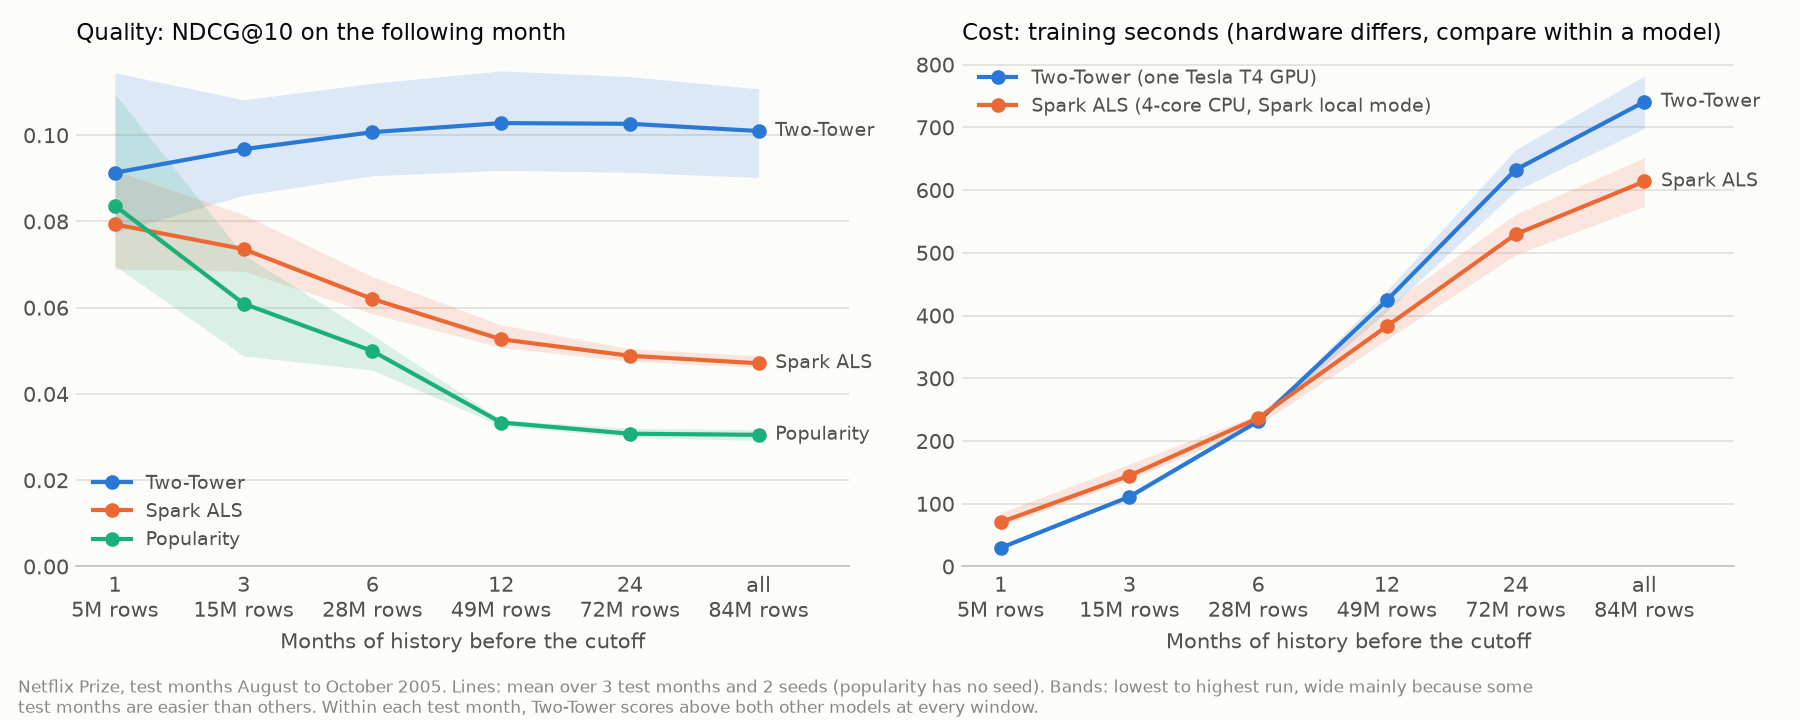
\includegraphics[width=\textwidth]{figures/history_windows.png}
\caption{Quality (left) and training time (right) against months of history before the cutoff.
Bands span the lowest to highest run; they are wide because some test months are easier than
others. Within each test month, the two-tower model scores above both other models at every
window. Training times come from different hardware and are compared only within a model.}
\label{fig:history}
\end{figure}

Table~\ref{tab:history} and Figure~\ref{fig:history} give the main result. The answer depends on
the model.

\emph{For popularity and ALS, more history is worse.} Both do best on the most recent month at
every test month, and for ALS every longer window scores lower at every test month. ALS on 1 month scores 1.68 times its
all-history score. At 1 month, ALS and popularity do not differ clearly: popularity is higher in
August and ALS in October. From 3 months up, ALS is higher at every test month.

\emph{The two-tower model needs about 6 months.} It improves up to 6 months and is then flat: its
6-month score is 98.0\% of its 12-month score, and the 1- and 3-month windows fall below the 95\%
line in at least one month. It does not gain beyond 12 months.

\emph{The neural model needs more history than ALS, and scores higher at every window.} By the
paired rule, the two-tower model is above both baselines at every window and test month. Its
smallest margin is 0.0038, over popularity on 1 month in August 2005, which is more than four
times either arm's standard error across users.

All five registered predictions held. The result is less surprising in light of an earlier
correction: before this experiment, ALS had been compared only with popularity over 12 months,
which it beat. A diagnostic run then showed that popularity over the last month alone beat both
tuned 12-month ALS models, at 0.0806 against 0.0491 for Spark ALS, 1.64 times as high. Beating
long-window popularity had been a weak test, and every later comparison included recent
popularity.

\subsection{What each month costs}

Training time grows with rows, not months. Spark ALS on all history took 8.68 times as long as
on 1 month (613.7\,s against 70.7\,s) for a lower score. For the two-tower model, 12 months took
1.83 times as long as 6 (424.4\,s against 231.6\,s) for a score within 5\%.

Storing ratings by month makes short windows cheaper to \emph{read}: in a registered benchmark,
monthly partitions cut the read time of a 3-month window by 75.6\% to 76.7\% against flat
Parquet. They did not clearly shorten \emph{training}: whole-job savings had overlapping ranges,
with medians of 1.2\% on 3 months and 3.5\% on 12 months, because reading is a small part of an
ALS job. The saving from a short window comes from training on fewer rows: a 3-month job took
65.1\% less time than a 12-month job. We therefore do not claim that partitioning shortens
training.

\subsection{Does Spark pay for itself on one machine?}

\begin{figure}[t]
\centering
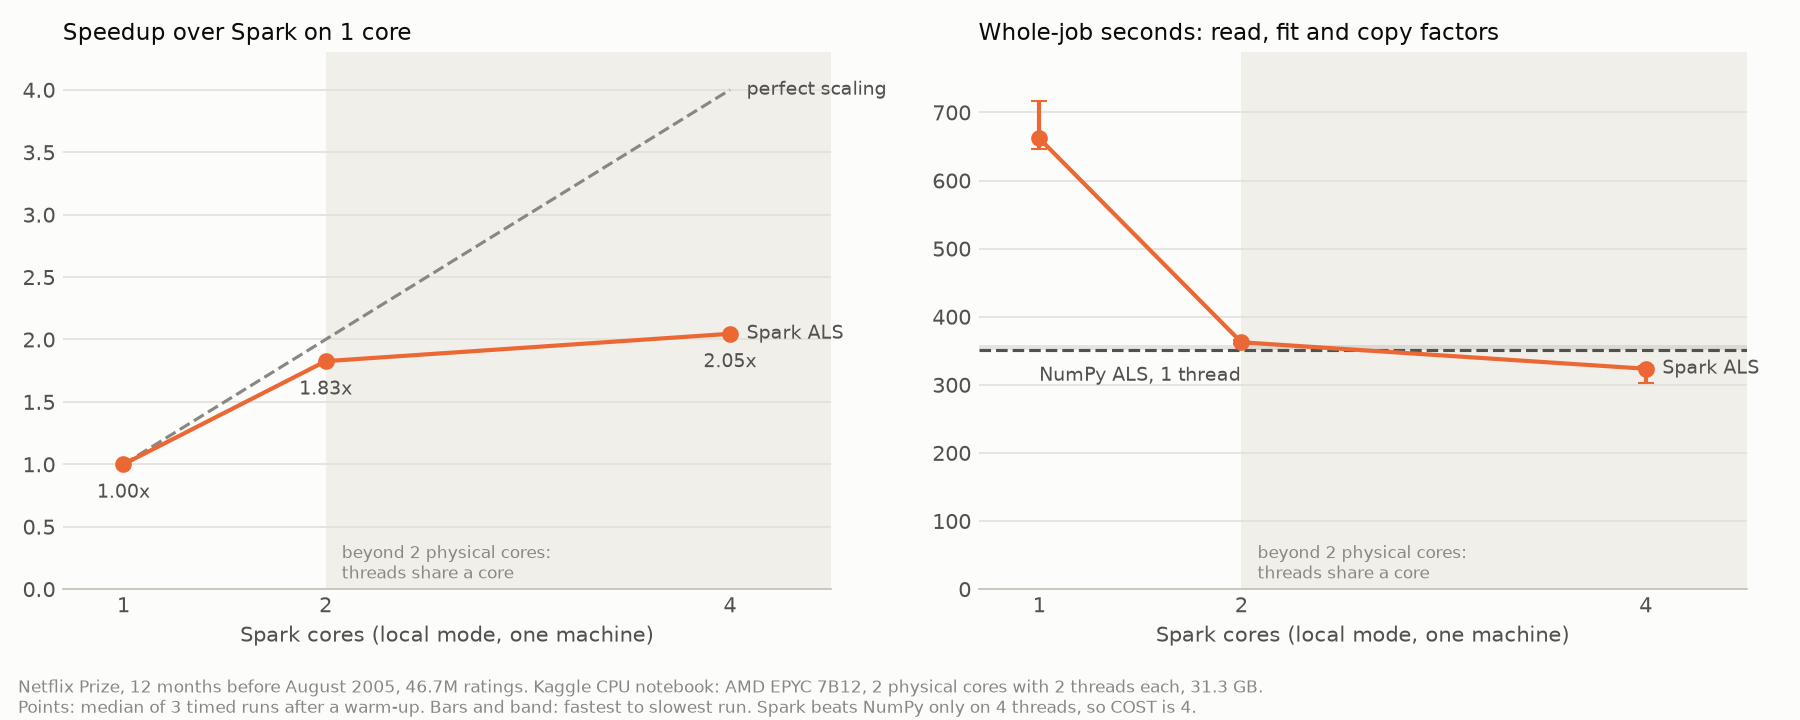
\includegraphics[width=0.85\textwidth]{figures/scaling.png}
\caption{Whole-job time for ALS on the 12 months before August 2005 (46,691,107 ratings), on a
Kaggle CPU notebook with 2 physical cores of 2 threads each. Spark runs in local mode.}
\label{fig:scaling}
\end{figure}

Because the main experiment used Spark, we measured whether it is needed. On the 12 months before
August 2005, with 1, 2 and 4 threads in local mode and three timed runs each
(Figure~\ref{fig:scaling}), Spark ALS took a median of 662.0\,s on 1 core, 362.5\,s on 2 and
323.6\,s on 4 threads: a speedup of 1.83 on the 2 physical cores and 2.05 on all 4 threads, which
share those cores. Single-threaded NumPy ALS doing the same job took 351.4\,s. Spark on one core
took 1.88 times as long, on 2 cores it was still 3.2\% slower, and only on all 4 threads did it
win, by a median of 7.9\%. Spark's COST for this job is therefore the whole machine. Its value
here is code that would run on a cluster, not speed on one machine. This measures threads in one
process, not a network of machines.

\subsection{Serving the model and its limit under load}

The two-tower model on 6 months before October 2005 was retrained for serving and scored 0.0993,
against 0.0994 in the main experiment. Evaluation and serving share one ranking function, and for
5,000 sampled users the service returned exactly the lists the evaluation scored. The service
uses NumPy over all 17,770 films, without an approximate index, and runs in a three-node
Kubernetes cluster created with kind on one laptop.

\begin{figure}[t]
\centering
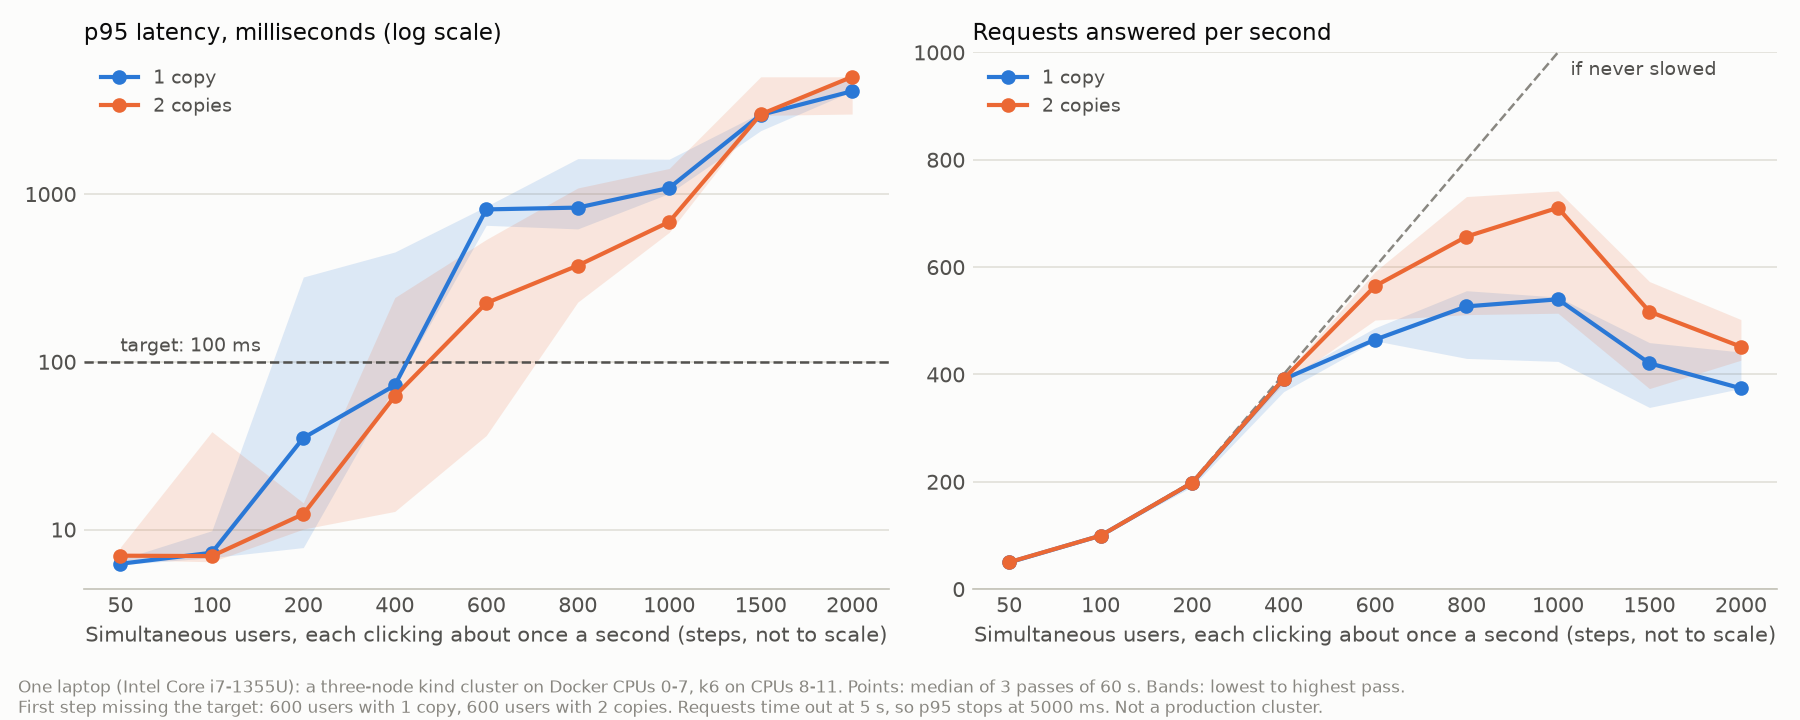
\includegraphics[width=\textwidth]{figures/load_test.png}
\caption{p95 latency (left) and requests answered per second (right) against simultaneous users,
for one and two copies of the service on one laptop (Intel Core i7-1355U). Points are medians of
three passes of 60\,s.}
\label{fig:load}
\end{figure}

A load test registered a target before any measured run: a 95th-percentile latency of at most
100\,ms with at most 1\% errors. The load generator ran on CPUs separate from the cluster's. With
one copy of the service, p95 latency was 6.3\,ms at 50 users and 72.4\,ms at 400 users, and the
target was missed at 600 (Figure~\ref{fig:load}). A second copy did not raise that limit. It
reached 1.32 times the peak requests per second of one copy, 710.5 against 540.0, below the
registered threshold of 1.5, and also missed the target at 600 users. Two of the three
predictions failed: we expected one copy to peak near 300 requests per second, and a second copy
to add more. One possible reason, not tested, is that one copy already uses more than one CPU:
the web framework serves requests on a pool of threads, and NumPy lets other threads run while it
computes. All parts shared one
laptop, so these numbers describe that laptop, not a production cluster.

\section{Threats to validity}

\paragraph{Narrow test period.} Three test months, all in late 2005, on one dataset. The finding
may not hold for other periods or services, and a second dataset was cut from scope.
\paragraph{Settings.} Settings were tuned on the 12-month window, which could favour it; that it
still lost for ALS makes this a conservative choice for the main finding. Fixed epochs give short
windows fewer training steps, which may understate the two-tower model on short windows.
\paragraph{Exposure.} Ratings reflect what Netflix showed its users. Some of the advantage of
recent history may come from what the service promoted, which this data cannot separate.
\paragraph{Offline measurement.} NDCG on held-out ratings rewards predicting what users rated, not
what they would have enjoyed, and favours popular films. No online test was possible.
\paragraph{Seeds and repeatability.} Two seeds per trained arm. GPU training was not bit-for-bit
repeatable across runs with the same seed, while NumPy ALS was.
\paragraph{Hardware.} Times come from shared, free notebooks and one laptop. Models on different
hardware are not compared by speed, Spark ran in local mode, and the load test's virtual users
wait for each answer, which understates queueing compared with real arrivals.

\section{Ethics and data handling}
\label{sec:ethics}

The Netflix Prize data was released as anonymous, and \citet{narayanan2008deanon} showed that a
few known ratings and dates could identify a subscriber's record. This project therefore does not
redistribute the data or any sample of it. The repository holds code, registered plans and
aggregate results only. The model bundle served in the cluster holds user IDs and their rated
films, so it is kept out of the repository and the container image, the service never logs a
user ID, and it returns film IDs without titles. Tests and continuous integration use synthetic
data. Recommenders trained on ratings also tend to favour popular films; this work measures
accuracy only and makes no fairness claim.

\section{Conclusion and future work}

How much history a recommender needs depends on the model. Popularity and ALS did best on the
most recent month and grew worse with more, while training time grew with every row. The
two-tower model needed about 6 months and gained nothing beyond 12. For all three models, history
beyond a year cost compute and bought no accuracy on these test months.

Natural next steps are a breakdown by user tenure and film popularity, more test months and a
second dataset, tuning each window separately, training for a fixed number of steps rather than
epochs, and testing whether an approximate index or several machines change the serving and
scaling results.

\paragraph{Reproducibility.} The code, registered plans, results, claims ledger and lab notebook
are public. \texttt{trs reproduce --sample} runs the whole method on synthetic data with a planted
change in user tastes on any laptop and checks that it is found; the full-data commands, each
with the commit its results record, are listed in \texttt{docs/REPRODUCING.md}.

\bibliographystyle{plainnat}
\bibliography{references}

\end{document}
